\documentclass[10pt,onecolcolumn,letterpaper]{article}
%% Welcome to Overleaf!
%% If this is your first time using LaTeX, it might be worth going through this brief presentation:
%% https://www.overleaf.com/latex/learn/free-online-introduction-to-latex-part-1

%% Researchers have been using LaTeX for decades to typeset their papers, producing beautiful, crisp documents in the process. By learning LaTeX, you are effectively following in their footsteps, and learning a highly valuable skill!

%% The \usepackage commands below can be thought of as analogous to importing libraries into Python, for instance. We've pre-formatted this for you, so you can skip right ahead to the title below.

%% Language and font encodings
\usepackage[spanish,english]{babel}
\usepackage[utf8x]{inputenc}
\usepackage[T1]{fontenc}
\usepackage{lipsum}
\usepackage{booktabs}


%% Sets page size and margins
\usepackage[a4paper,top=3cm,bottom=2cm,left=3cm,right=3cm,marginparwidth=1.75cm]{geometry}

%% Useful packages
\usepackage{amsmath}
\usepackage{graphicx}
\usepackage[colorinlistoftodos]{todonotes}
\usepackage[colorlinks=true, allcolors=blue]{hyperref}

%% Title
\title{
		%\vspace{-1in} 	
		\usefont{OT1}{bch}{b}{n}
		\normalfont \normalsize \textsc{Privacy and Big Data} \\ [10pt]
		\huge GNUmed \\
}

\usepackage{authblk}

\author[1]{Antoine Janssens}
\author[1]{Maria Karegla}
\author[2]{Michiel Creemers}
\author[2]{Yosra Ben Taarit} 

\affil[1]{\small{Advanced Master's in Cybersecurity}}
\affil[2]{Master of Artificial Intelligence}

\begin{document}
\maketitle

\selectlanguage{english}
\begin{abstract}

\end{abstract}


{\textbf{Keywords} \\
Big Data, Health, Privacy, GNU, open-source} %TO DO: find bether words

\section{Introduction}
% \lipsum[40]
\begin{figure}[h!]
    \centering 
    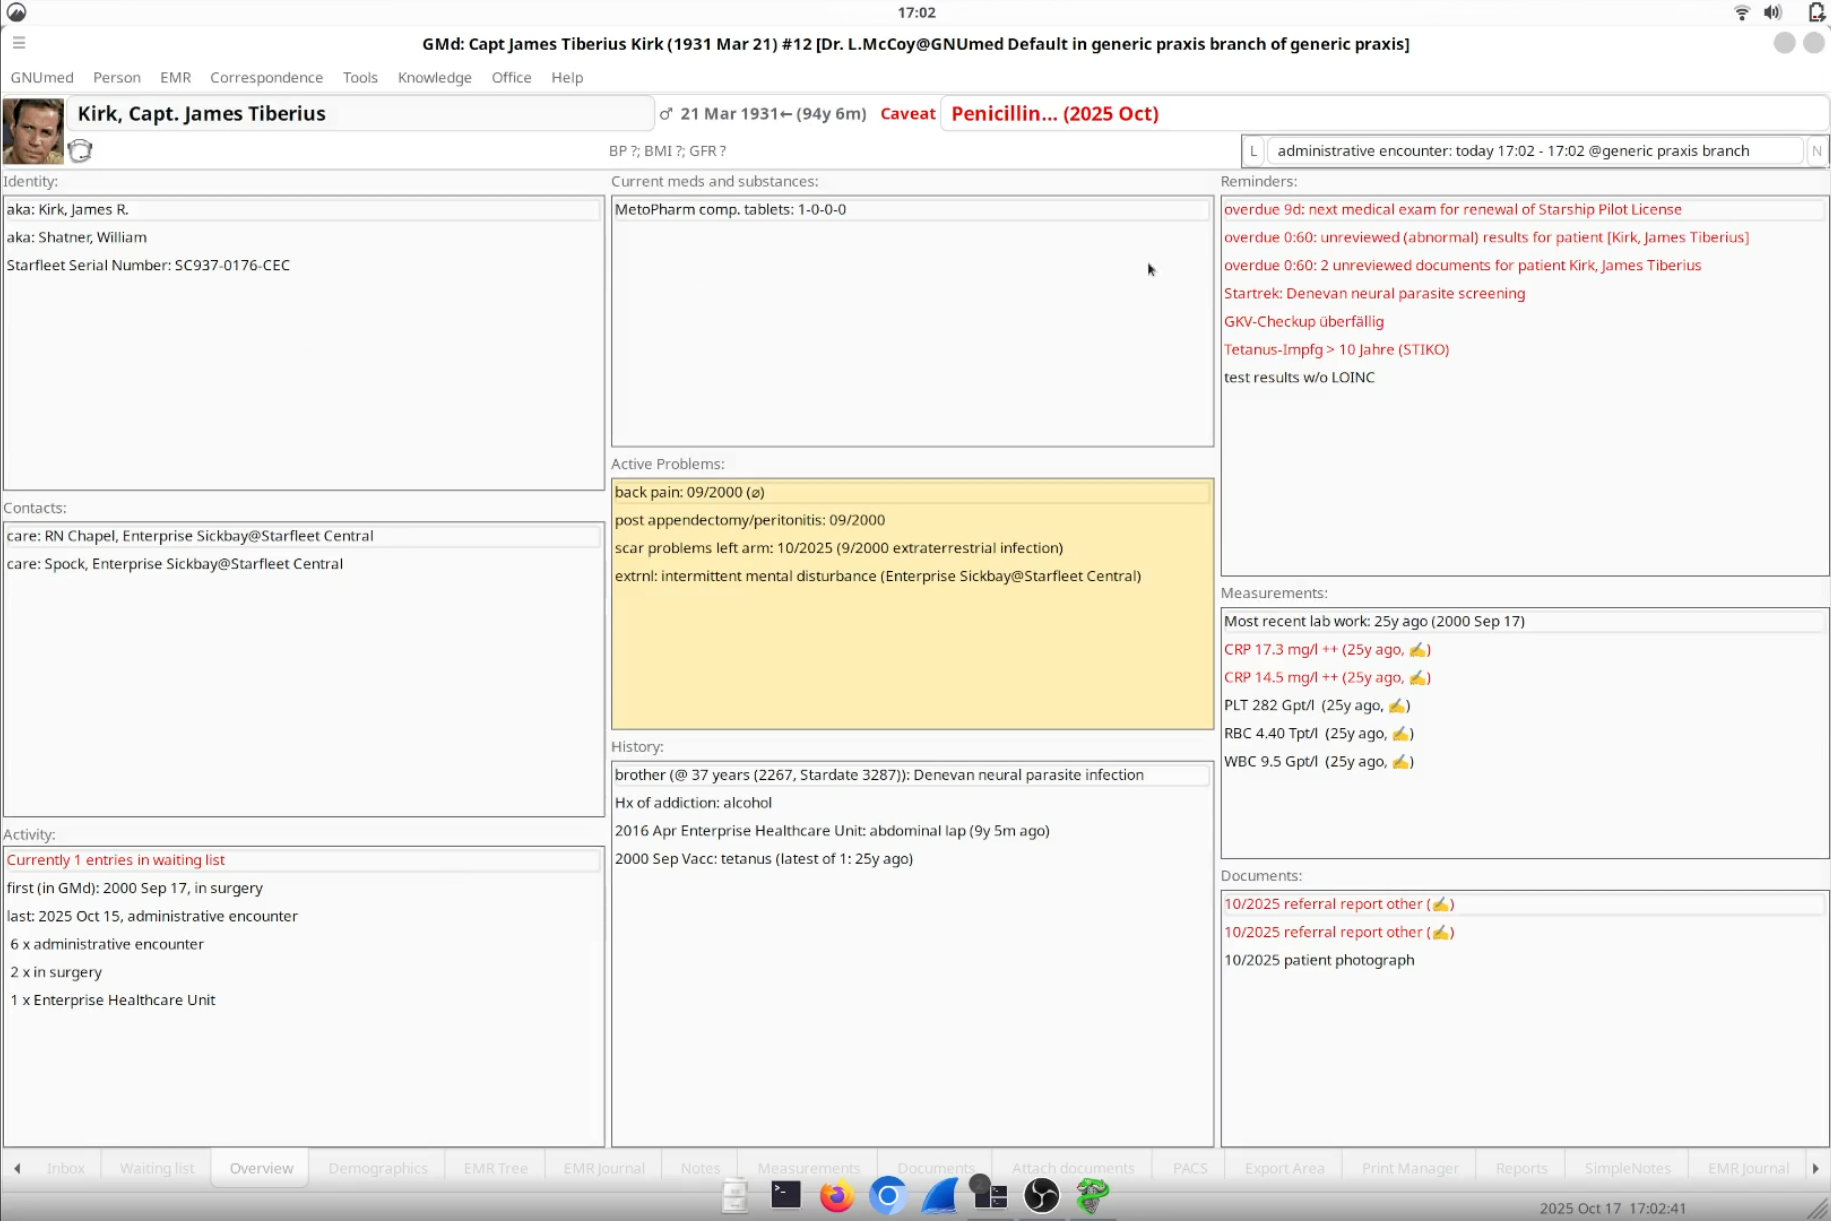
\includegraphics[width=0.8\textwidth]{Screenshot_Gnumed.png}
    \caption{GNUmed Screenshot of patient file. }
    \label{fig:gnumed_screen_img} 
\end{figure}

\section{Technical description of the system}
\subsection{System Architecture}

Based on the GNUmed introduction document\cite{gnumed_development_team_gnumed-introduction_v4pdf_2005}, we deduct that GNUmed makes use of a flexible client-server model. Thigh high-level component diagram details their key responsibilities.

The \textbf{GNUmed Client} consists of the main GNUmed application. A Database Service Broker is used to abstract the backend service distribution. This provides a unified data source that the rest of the application can make use of, providing transparency to the physical layout for user and developer alike. In adherence with security requirements, a client side cryptography engine handles the encryption of sensitive data, ensuring that even before being transmitted, the data of this nature cannot be accessed. 

The \textbf{GNUmed Backend} is built on a PostgreSQL database and is not monolithic. It is made up of a collection of distributed services. Data that is related is regarded as a service and hence can be treated as a logical component. Services are not necessarily present on the same physical server. Within the database, business logic if enforced through the use of triggers. These triggers also maintain an Audit Trail, as required legally, by automatically capturing all changes, by keeping copies of the unchanged instances. The tables are highly normalized in order to optimize storage. For the client, data access is simplified through an abstraction layer of updateable views, which sit on top of the tables. Access to these data is managed through a user hierarchy that regulates permissions. 

Finally, the \textbf{Communication} between the client and server is secured using industry standard protocols, with examples being SSL for encryption and Kerberos for authentication. The architecture also allows for \textbf{Optional Middleware}, to be placed between client and backend, allowing for more complex integrations or business logic external to the database.

\subsection{The Logical Data Model}

The system's UML Class Diagram as shown in Figure \ref{fig:uml_image}, represents the logical data model and details the structure of the data located in the PostgreSQL backend. The figure is outdated and is lacking information. It provides a blueprint for some of the services, as previously described, with each prefix corresponding to a specific schema and hence a service. In this case we have the \texttt{Demographic Service}, represented by \texttt{dem.}, \texttt{Clinical Service} by \texttt{clin.}, \texttt{Document Storage Service} represented by \texttt{blobs.} and \texttt{German Specific Schema} represented by \texttt{de\_de.}

\begin{figure}[h!]
    \centering 
    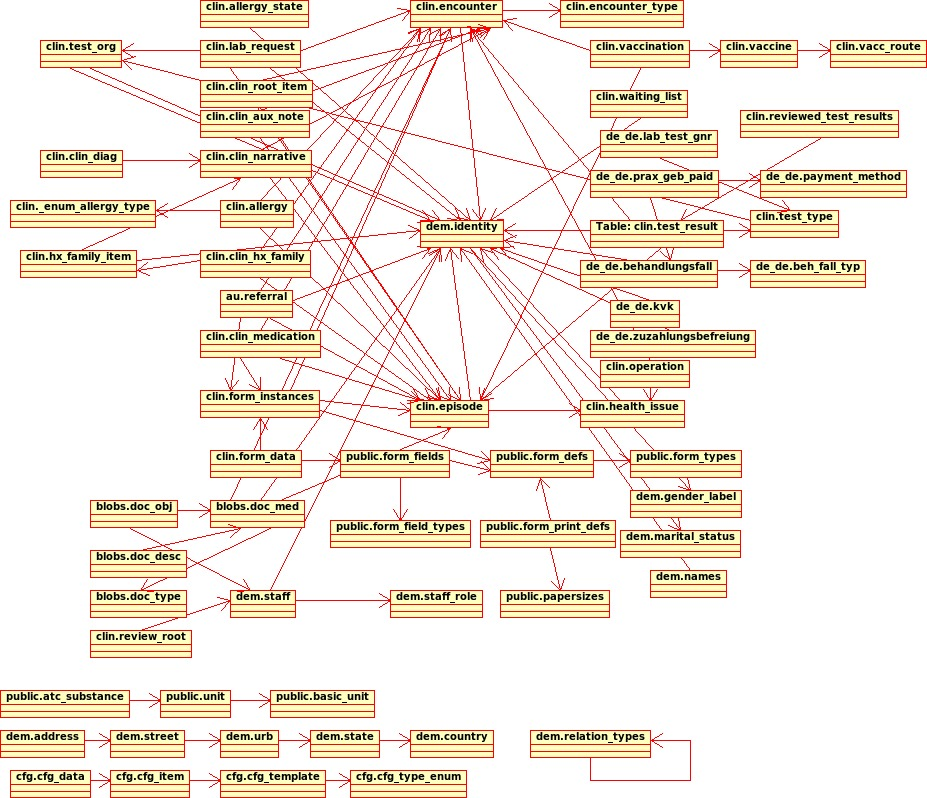
\includegraphics[width=0.8\textwidth]{uml.jpg}
    \caption{GNUmed UML Class Diagram. Note: outdated (~2002) and missing elements \cite{res_medicinae_domainpng_nodate} }
    \label{fig:uml_image} 
\end{figure}













% \begin{table}[h!]
% \centering
% \caption{System Architecture Components}
% \label{tab:system_architecture}
% \begin{tabular}{l l p{7cm}}
% \toprule
% \textbf{Layer} & \textbf{Component} & \textbf{Description} \\
% \midrule
% Frontend       & GNUmed Client      & Python GUI, handles user interaction \\
% Middleware     & Optional Services  & For integration, data exchange, or remote control \\
% Backend        & PostgreSQL DB      & Stores patient records, audit logs, medical data \\
% Plugins        & Custom Modules     & Extend functionality (e.g., lab results, imaging) \\
% External Tools & Scanners, DICOM viewers & Integrated via Python bindings or shell scripts \\
% \bottomrule
% \end{tabular}
% \end{table}







\section{technical privacy issues}
%TO DO: issues from the diagram
% \lipsum[60]

\section{technological recommendations}

% \lipsum[60]

% example code
% {\scriptsize
% \begin{verbatim}
% \begin{figure}
%     \centering
%     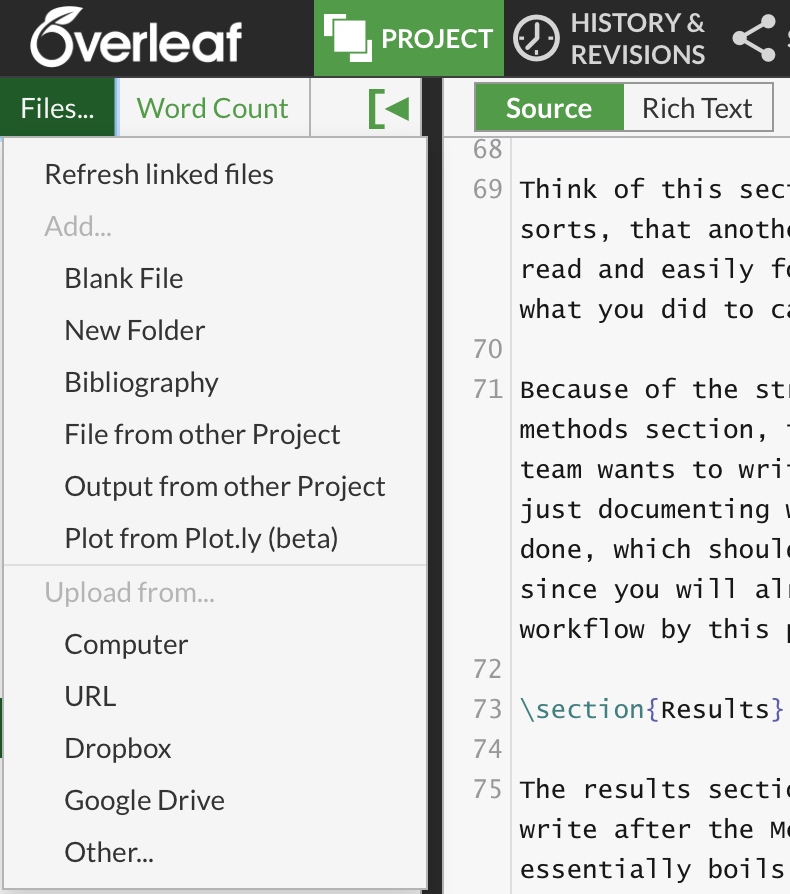
\includegraphics[width=0.4\textwidth]{test.png}
%     \caption{Hello!}
% \end{figure}
% \end{verbatim}
% }

%example figure
% \begin{figure}
%   \centering
%   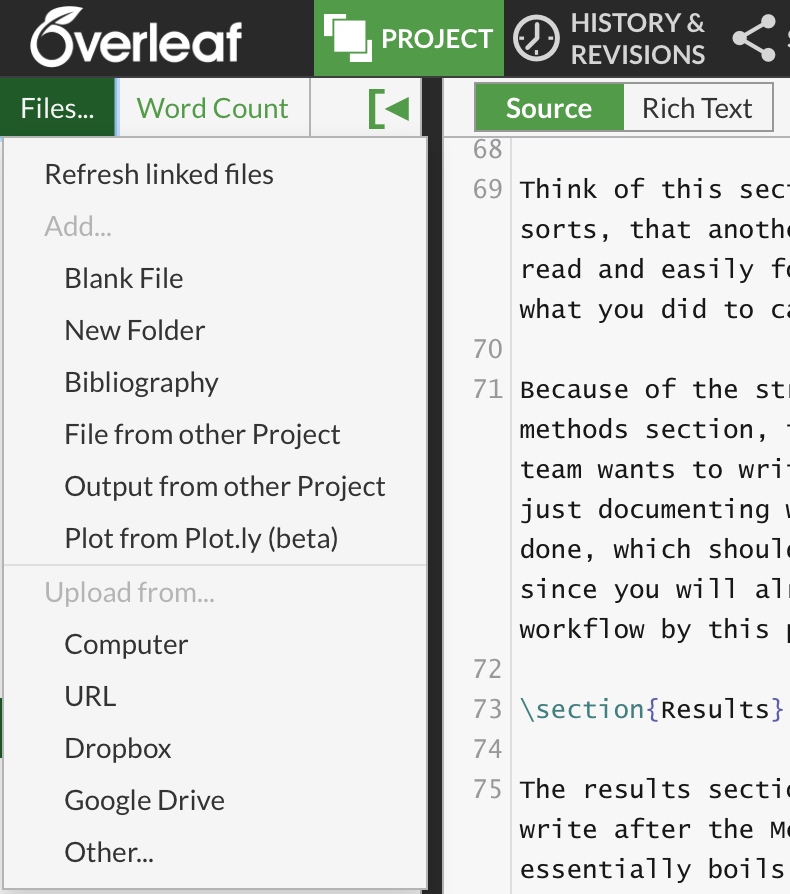
\includegraphics[width=0.4\textwidth]{test.png}
%   \caption{Notice how \LaTeX\ automatically numbers this figure.}
% \end{figure}

% \section*{Conclusions}
% \lipsum[30]

% \section*{Acknowledgements}
% Anyone to thank/credit for helping your team along the way? This is the place to do it.



\bibliographystyle{plain}
\bibliography{references}


\end{document}